The lepton momentum scale and resolution, and the missing energy scale and
resolution are studied by comparing $\dyll$ data and simulated events, and
applying an additional correction to the simulation to agree with the values 
in data. The corrected values are used to assign the corresponding 
uncertainties. The obtained values are not intended to be high precision 
measurements, but a realistic way of assigning the uncertainties. 
$\dyll$ events are selected by requiring two and only two opposite-sign
same-flavor leptons with a dilepton mass between 82 and 100 $\GeV$. Events are
rejected if they are b-tagged to reduce the contamination from top background.

For the lepton momentum scale and resolution studies, we compare the dilepton
mass and apply a correction to the lepton scale and to the resolution in the
simulation to agree with the data. The correction factors depend on the lepton
flavor, and if the lepton is in the barrel or endcap regions. The distributions for
the data, the uncorrected simulation and the corrected simulation are shown in
Fig.~\ref{fig:test_lep_zll}.

For the missing energy scale and momentum, events are split in jet 
multiplicities: 0-jets, 1-jet and $\geq$2-jets bins. The X and Y components of
both standard missing energy and track missing energy are compared between data
and simulation. The distributions for the data, the uncorrected simulation and 
the corrected simulation are shown in Figs.~\ref{fig:test0_met_zll},
~\ref{fig:test1_met_zll}, and~\ref{fig:test2_met_zll}, for 
0-jets, 1-jet and $\geq$2-jets bins, respectively.

\begin{figure}[hbt]
\begin{center}
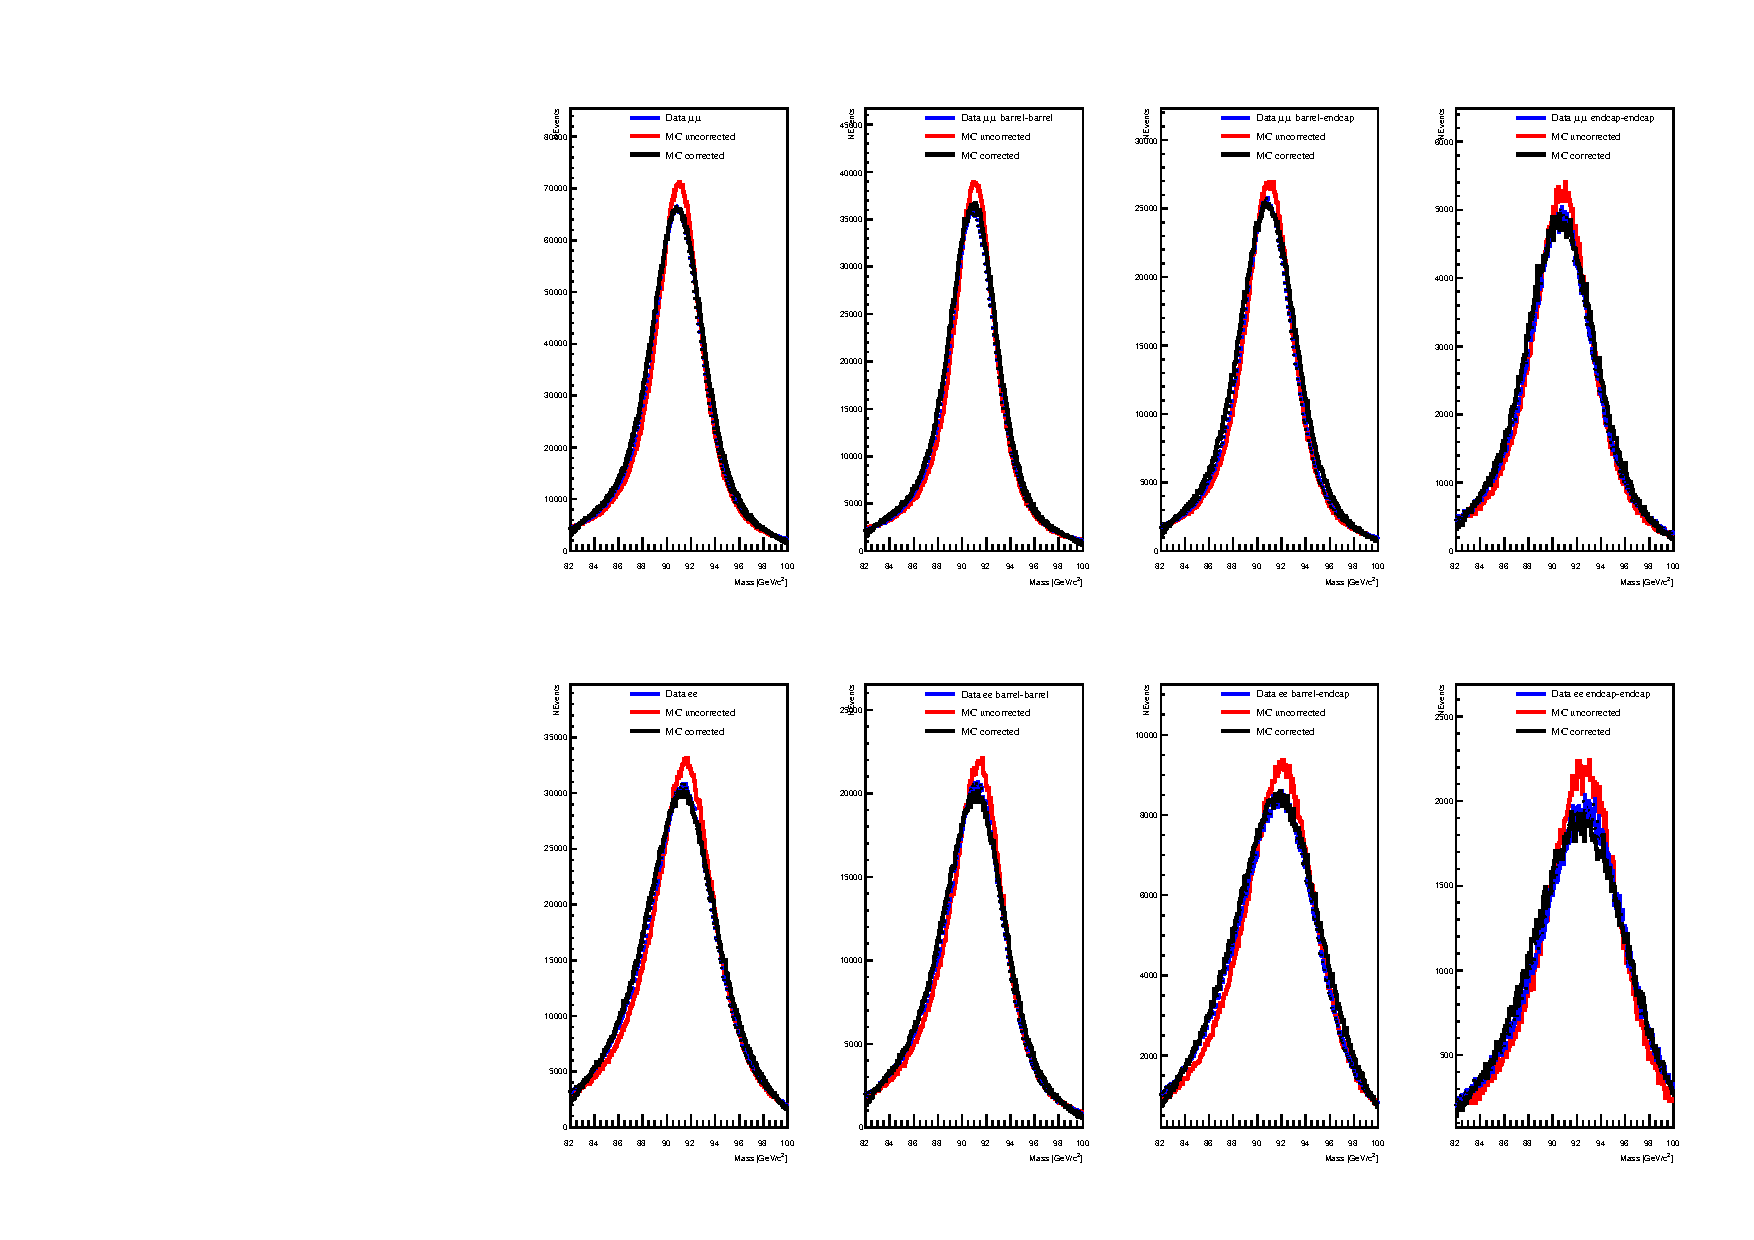
\includegraphics[width=0.75\linewidth]{figures/test_lep_zll.pdf} 
\caption{\label{fig:test_lep_zll} Dilepton mass distribution in 
data, uncorrected simulation and corrected simulation on $\dyll$ events.}
\end{center}
\end{figure}

\begin{figure}[hbt]
\begin{center}
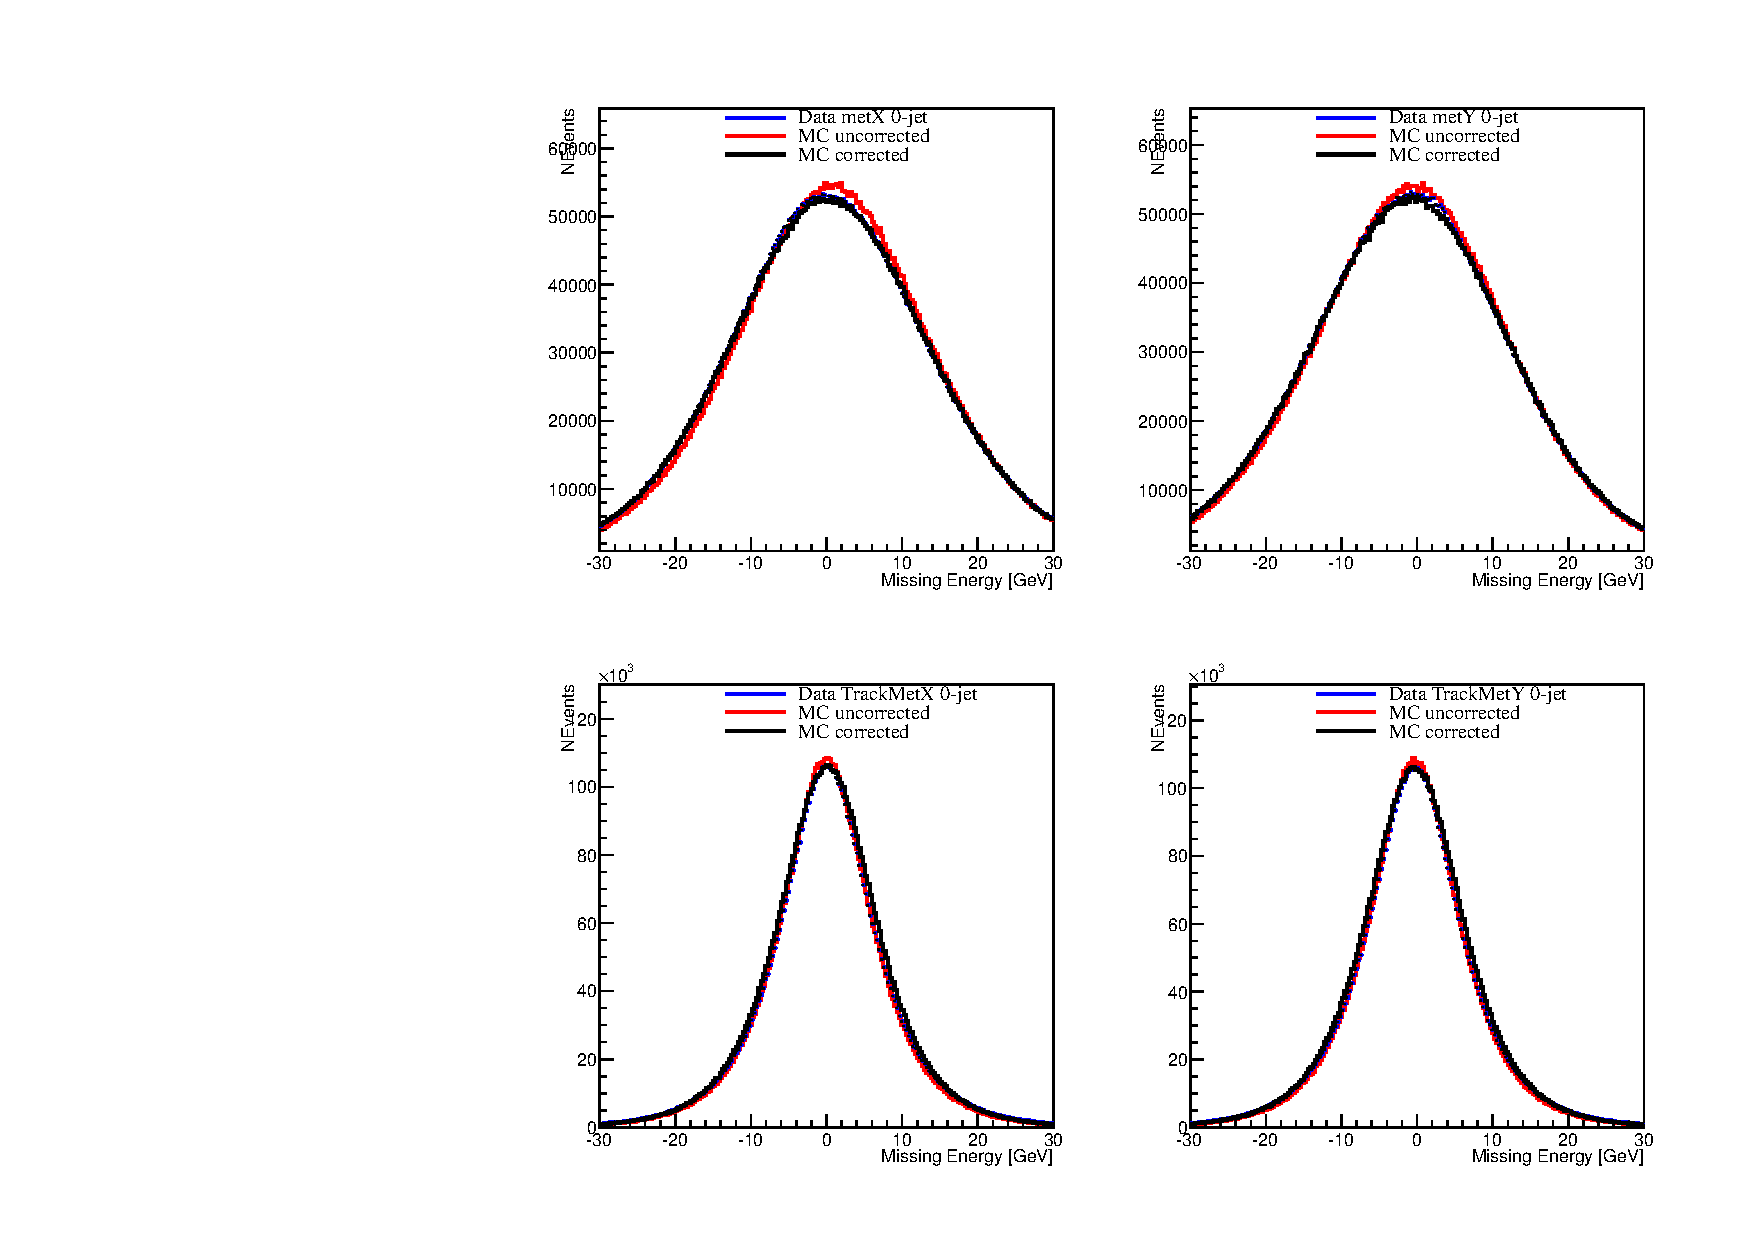
\includegraphics[width=0.75\linewidth]{figures/test0_met_zll.pdf} 
\caption{\label{fig:test0_met_zll} Missing energy on data, 
uncorrected simulation and corrected simulation on $\dyll$ events in 
the 0-jet bin.}
\end{center}
\end{figure}


\begin{figure}[hbt]
\begin{center}
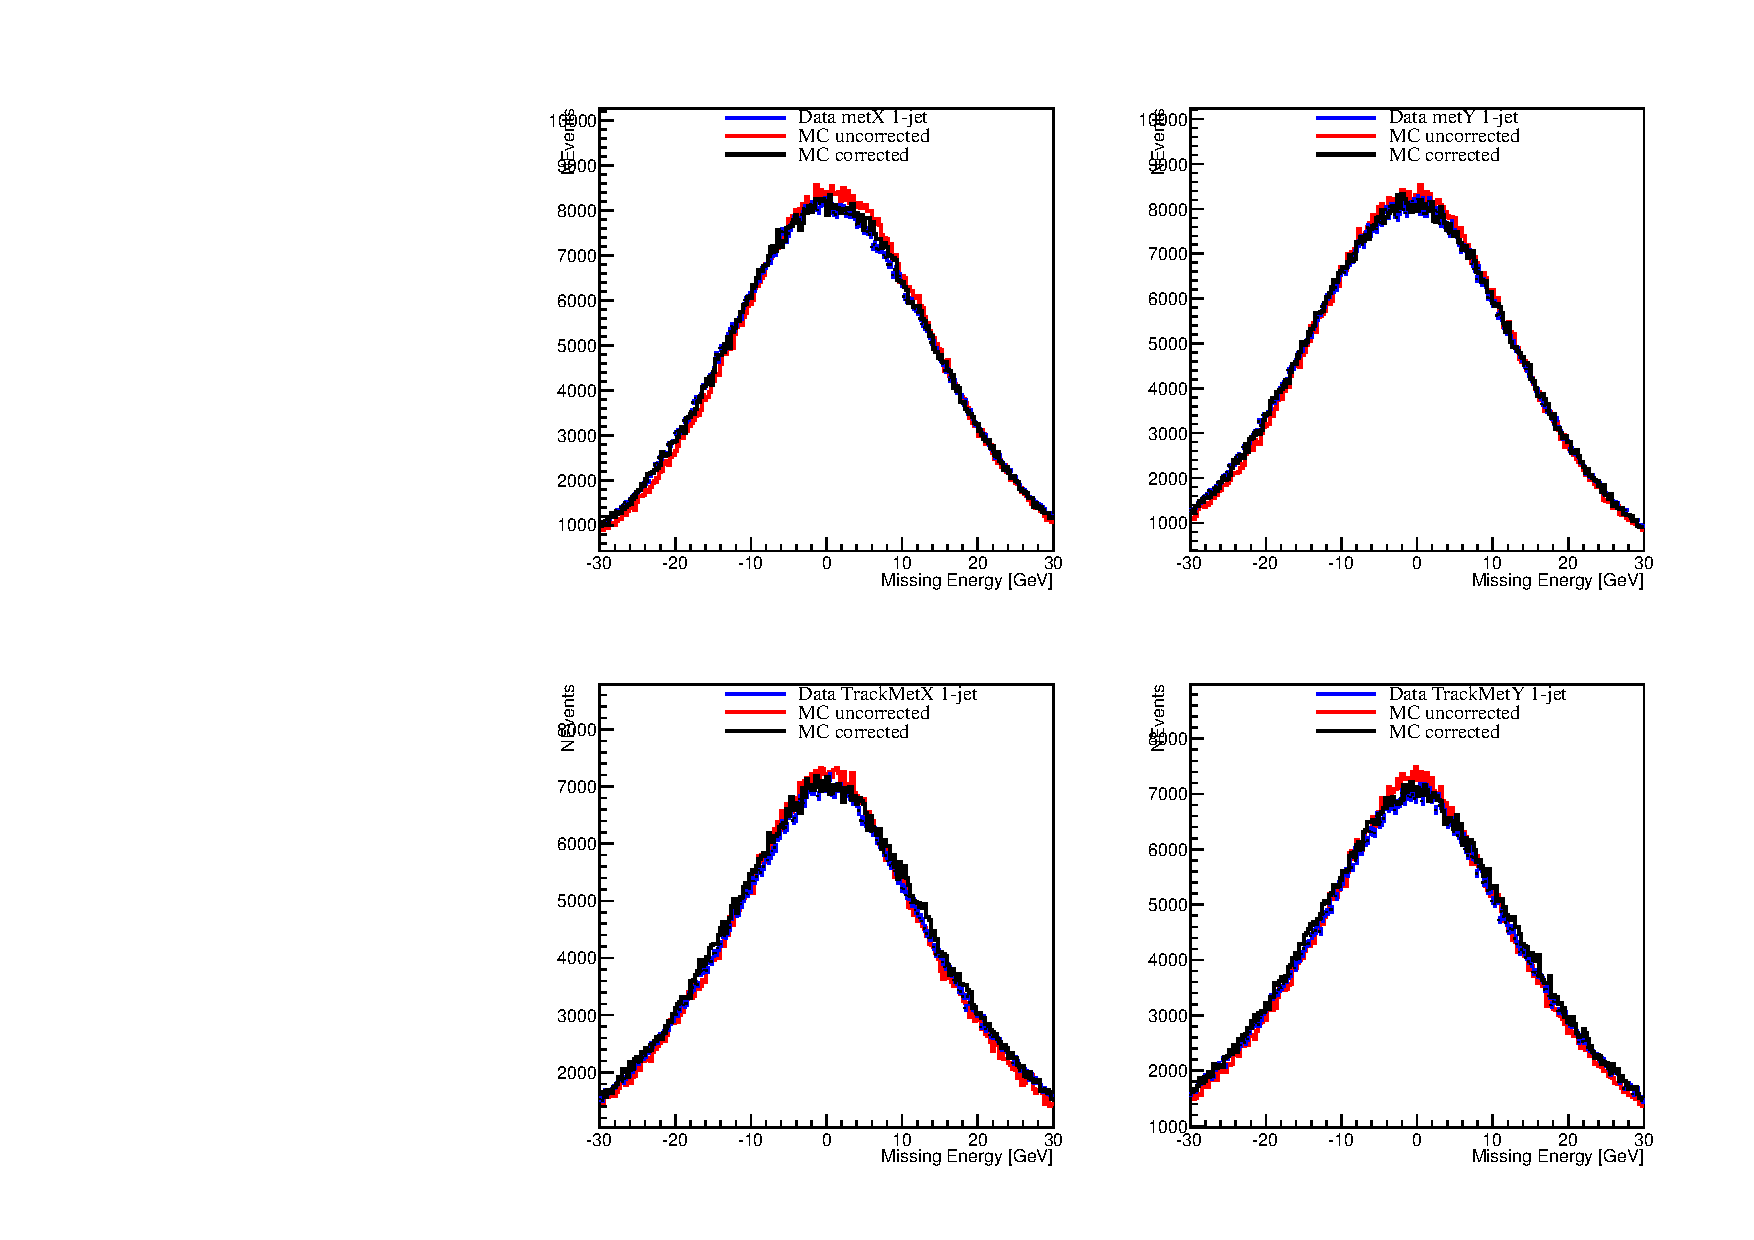
\includegraphics[width=0.75\linewidth]{figures/test1_met_zll.pdf} 
\caption{\label{fig:test1_met_zll} Missing energy on data, 
uncorrected simulation and corrected simulation on $\dyll$ events in 
the 1-jet bin.}
\end{center}
\end{figure}

\begin{figure}[hbt]
\begin{center}
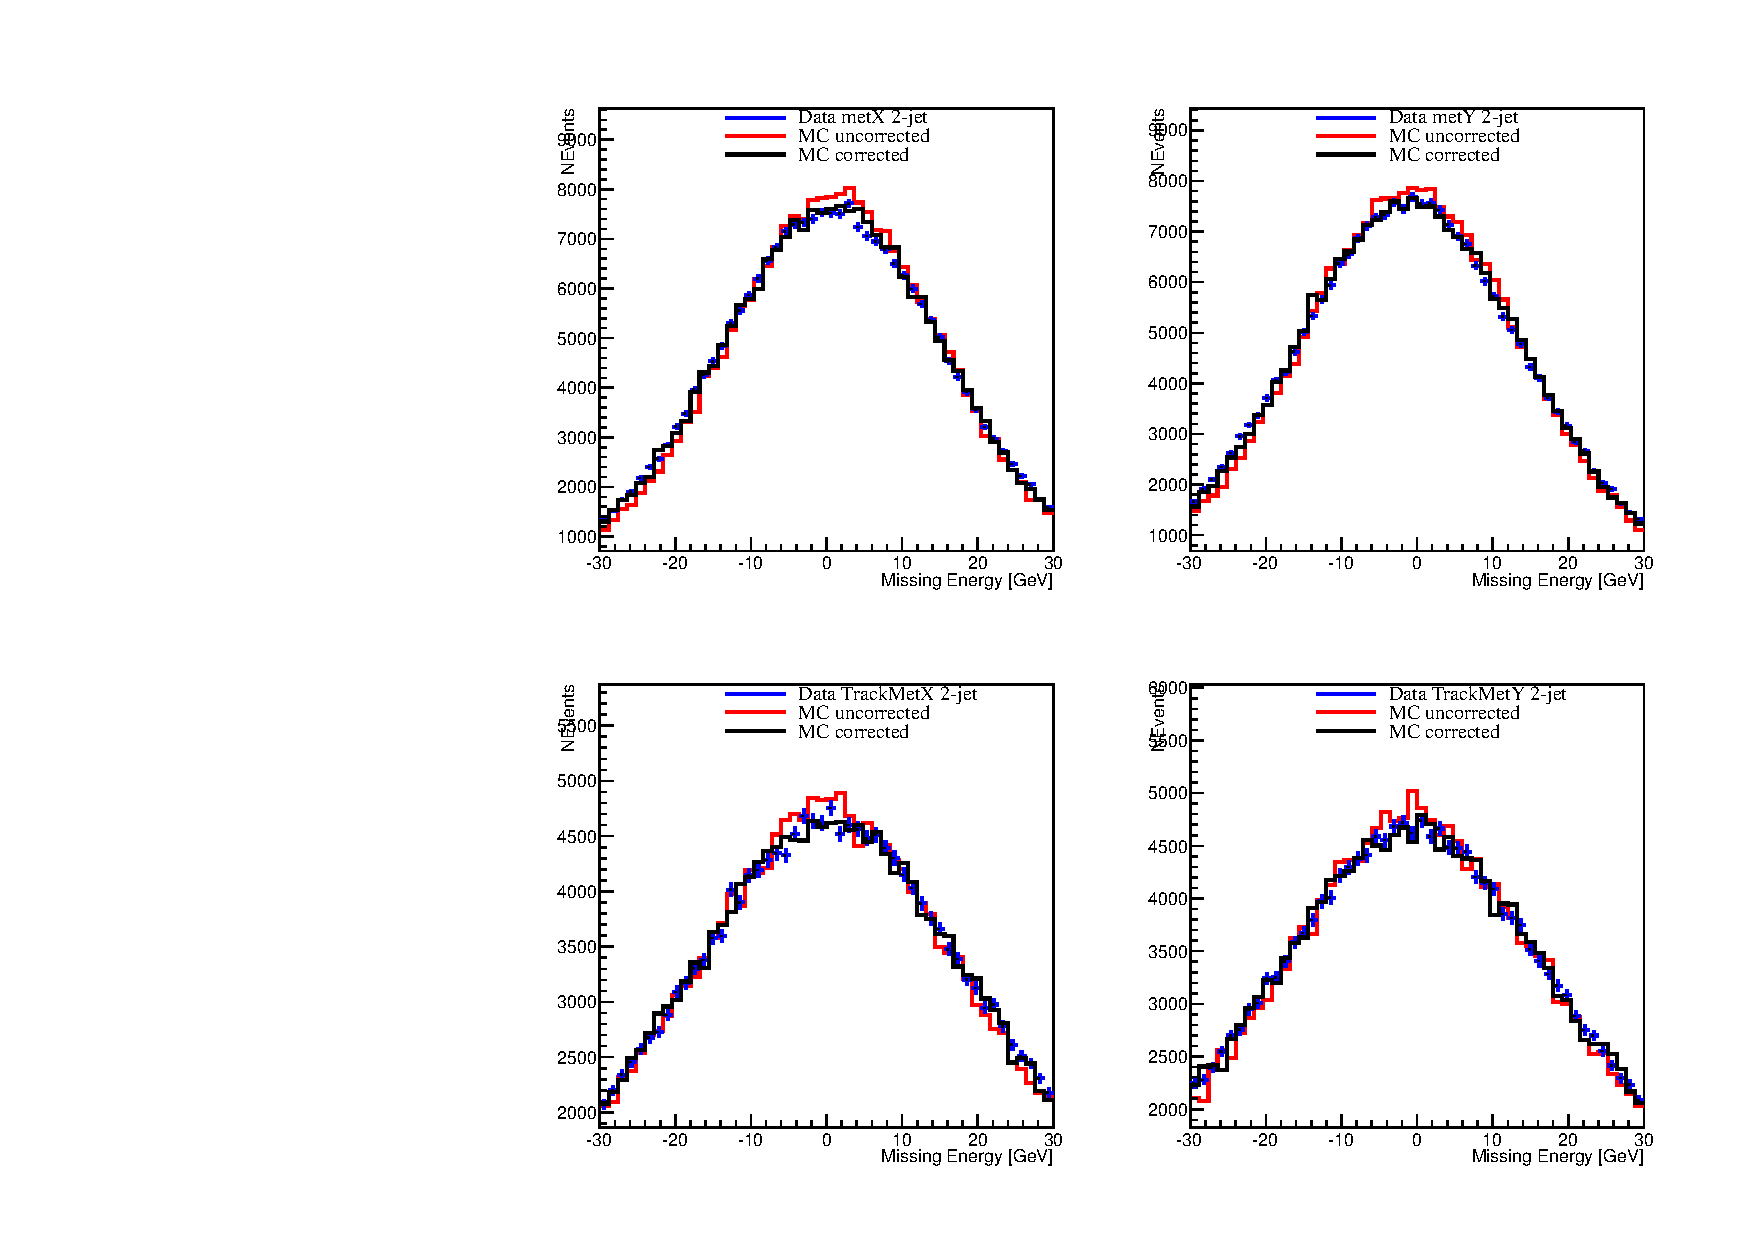
\includegraphics[width=0.75\linewidth]{figures/test2_met_zll.pdf} 
\caption{\label{fig:test2_met_zll} Missing energy on data, 
uncorrected simulation and corrected simulation on $\dyll$ events in 
the $\geq$2-jet bin.}
\end{center}
\end{figure}


